\DeclareUnicodeCharacter{2028}{} 
\documentclass{article}
\usepackage{blindtext}
\usepackage[section]{placeins}
\usepackage[T1]{fontenc}
\usepackage[utf8]{inputenc}
\usepackage{titling}
\usepackage{float}
\usepackage{tikz}
\usetikzlibrary{calc}
\usetikzlibrary{arrows.meta}
\usepackage{graphicx}



\title{ Requirement Analysis and Specification Document\\2020-2021}
\author{Alessandro Polidori (Codice persona 10573078)\\Olimpia Rivera (Codice persona 10617517)}
\date{}



\renewcommand{\contentsname}{Table of Contents}


\begin{document}

\renewcommand{\labelitemi}{\normalfont -}

\begin{figure}[]
  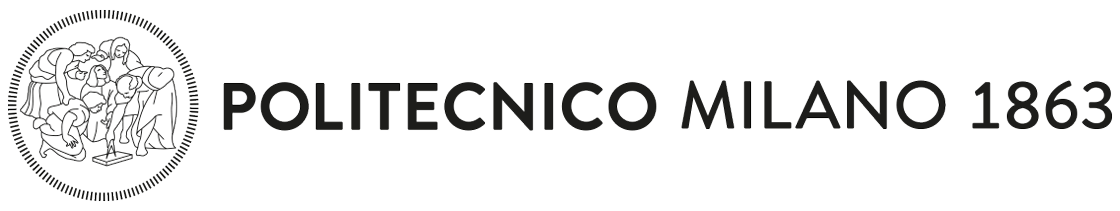
\includegraphics[width=\linewidth]{logo_politecnico.png}
  
\end{figure}
\maketitle
\tableofcontents{}

\newpage

\section{Introduction}

\subsection{Purpose}
This document provides an analysis of the system in terms of assumptions, functional and non functional requirements needed to fulfill its main goals. It describes the domain in which the system will be deployed by presenting relevant scenarios and use cases and it highlights the software’s limits and constraints.
\bigskip\\
The document is addressed to all the stakeholders affected by the software and is meant to be used by developers in order to realize a system that meets the purpose for which it was intended.\\

\subsection{Scope}
\subsubsection{Description of the given problem}
The CLup system is designed to regulate accesses to stores and manage lines in real time in order to respect restrictions imposed by the virus emergency and avoid crowds and long lines. In particular, the software is offered to both stores managers to monitor the influx of people in their buildings and to common users, allowing them to virtually “line-up” from home and book visits to the stores.\\
\smallskip\\
The main functionalities offered by CLup are the following:\\
\begin{itemize}
\item Basic service: allows stores' customers to line up from home and to approach the store only when their turn is about to arrive. In order for this lining up mechanism to work effectively, the software generates an estimation of the waiting time and alerts users when is the moment to reach the store, taking into account the time they need to get to the shop from the place they are located. The estimated time is calculated considering the number of people in the virtual line and the time spent inside the store by the costumers that are already shopping. The system is also able to optimize or increase the waiting times of users in the queue when needed. In addiction, when customers enter and exit the stores, a QR code generated by the application is scanned, allowing store managers to monitor the influx of people.
\item Advanced service: allows users to book a time-slot to visit the store. When booking, users can provide the categories of the items that they intend to purchase. The system will be able to manage visits in a finer way taking into account the store's departments that customers are going to occupy.
\end{itemize}
When customers line up or make a slot reservation they are asked to provide the expected duration of the visit. Alternatively, they can let the software itself infer it (this works only for long-term customers by analyzing the customer’s previous visits).
Be aware that the functions described above will be further detailed in the next sections of the document.
\subsubsection{World Phenomena}
\noindent\medskip
[WP1] - Stores’ customers either owning or not a smartphone.\\
\noindent\medskip
[WP2] - Customers approaching the store.\\
\noindent\medskip
[WP3] - Customers arriving too early at the shop for unexpected reasons.\\
\noindent\medskip
[WP4] - Customers doing the shopping.\\
\noindent\medskip
[WP5] - Customers walking away from store.
\subsubsection{Shared Phenomena}
\noindent\medskip
[SP1] - User enters the store (QR code scanned) - World controlled.\\
\noindent\medskip
[SP2] - User gets in line - World controlled.\\
\noindent\medskip
[SP3] - System shows number and estimated waiting time - Machine controlled.\\
\noindent\medskip
[SP4] - System generated QR code and line number - Machine controlled.\\
\noindent\medskip
[SP5] - System notifies the user to reach the store - Machine controlled.\\
\noindent\medskip
[SP6] - System updates waiting time - Machine controlled.\\
\noindent\medskip
[SP7] - User doesn't arrive in time - World controlled.\\
\noindent\medskip
[SP8] - User cancels reservation (either slot or line) - World controlled.\\
\noindent\medskip
[SP9] - User books a slot - World controlled.\\
\noindent\medskip
[SP10] - User indicates expected duration of visit or requests system to infer it - World controlled.\\
\noindent\medskip
[SP11] - User makes list of items - World controlled.\\
\noindent\medskip
[SP12] - User exits the store (QR code scanned) - World controlled.\\
\subsubsection{Goals}
\noindent\medskip
[G1] - Provide customers a safe environment in the stores.\\
\noindent\medskip
[G2] - Manage virtual lines in order to avoid the formation of long lines outside stores.\\
\noindent\medskip
[G3] - Allow store managers to monitor the influx of people in their buildings.\\
\noindent\medskip
[G4] - Allow users to book slots for visiting the store.\\
\noindent\medskip
[G5] - Allow users to arrive on time for their turns.\\
\subsection{Definitions, Acronyms, Abbreviations}
\subsubsection{Definitions}
\begin{itemize}
\item Product type: a set of similar products. Usually, items with the same product type are located in the same store's department
\item Smart Turnstile: a turnstile equipped with a QR codes scanner
\item Store's department: a specific section of the store, containing only a subset of all the product types
\item Store manager: the person responsible for the store and for the interactions between the store and the system. He can be helped by his employees
\item Waiting time: an estimation of the time needed to the queue to get to a specific turn number
\end{itemize}
\subsubsection{Acronyms}
\begin{itemize}
\item GPS: Global Positioning System
\item API: Application Programming Interface
\end{itemize}
\subsubsection{Abbreviations}
\begin{itemize}
\item WPn: n-th World Phenomena
\item SPn: n-th Shared Phenomena
\item Gn: n-th Goal
\item Dn: n-th Domain Assumption
\item Rn: n-th Functional Requirement
\end{itemize}
\subsection{Reference Documents}
\subsection{Overview}
The RASD document is structured in the following 5 chapters:
\begin{itemize}
\item\textbf{Chapter 1} describes the document’s purpose and brief identification of the context in which the application is going to work given its main functionalities. It also provides lists of world phenomena, shared phenomena and goals that the system is supposed to achieve. Finally, useful specifications (definitions, acronyms, abbreviations) are included for a better understanding of the next sections of the document.
\item\textbf{Chapter 2} gives an overall description of the project. The class diagram in the Product Perspective provides a conceptual overview of the main elements of the system and the state charts describe the evolution of relevant objects. In the Product Function section, the system’s high level functionalities are further detailed and clarified. The expected type of actors that will interact with the system are listed in User Characteristics. Ultimately, chapter 2 describes the system’s constraints and the domain properties assumed to hold in the world.
\item\textbf{Chapter 3} describes the external interface requirements (user, hardware and software interfaces). Some scenarios are listed to clarify how the system works in real world situations. Both functional and non-functional requirements are described. The former are defined by several use cases and their relatives sequence diagrams, while the latter are identified though performance requirements, design constraints and software system attributes.
\item\textbf{Chapter 4}
\item\textbf{Chapter 5}
\end{itemize}


\section{Overall Description}
\subsection{Product Perspective}
\subsubsection{Class diagram}
The class diagram below gives a high level representation of the system's domain. Classes contains only the necessary attributes to highlight the most important dynamics. \textbf{QR Code} is associated either to a \textbf{Turn Number} or to a \textbf{Reservation} and is provided with attributes required to associate the measured duration of the stay to the user. Reservation contains a list of \textbf{Product Types} and every product type is located in a specific store \textbf{Department}. A \textbf{Queue} is composed by a certain amount of \textbf{Turn numbers}. The \textbf{Distance} needs two \textbf{Positions} and can access to the time estimated by the \textbf{Maps Service API}. Also, \textbf{Customer} has a direct access to a list of the previous shopping times (calculated by the system using \textbf{QR Code} attributes).\newline\newline\newline\newline
\begin{figure}[H]
  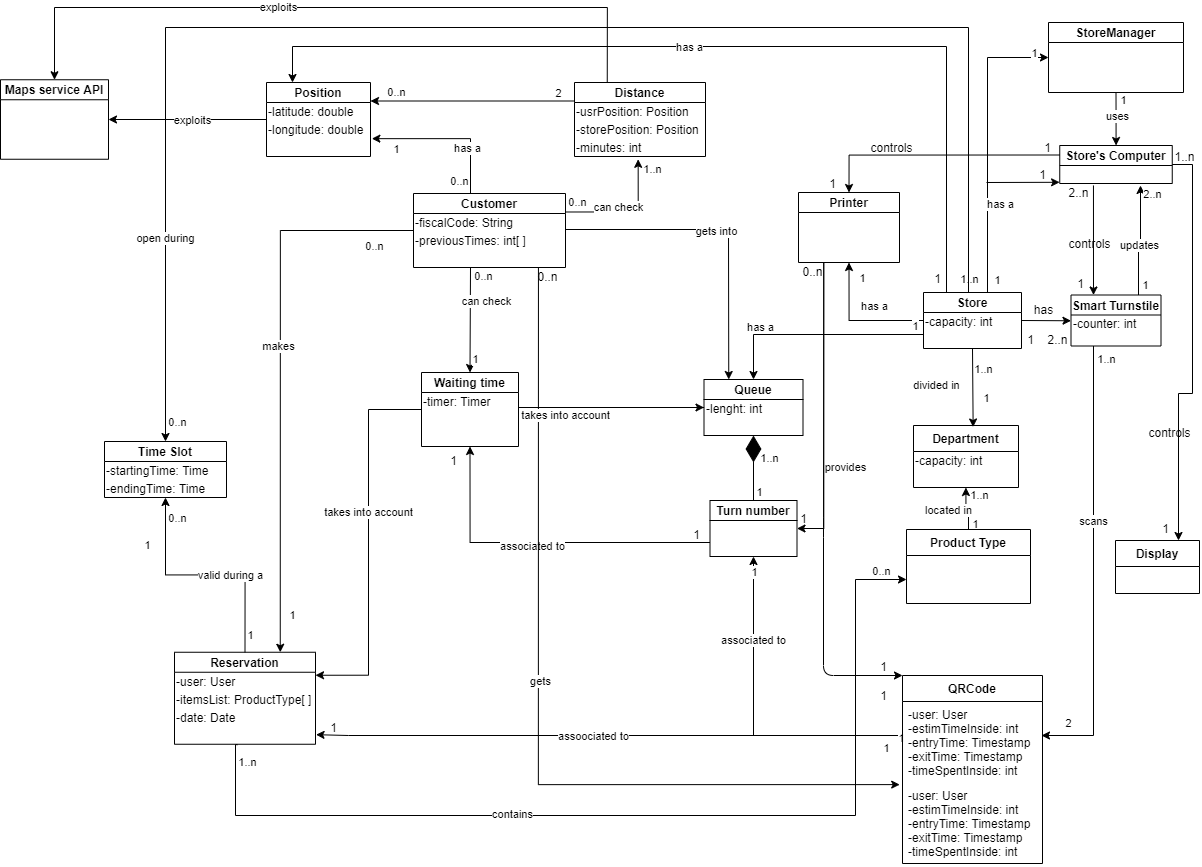
\includegraphics[width=\linewidth]{class_diagram.png}
  
\end{figure}

\newpage
\subsubsection{Statechart diagrams}

The diagrams below represent the states relative to some classes we wanted to analyse.

\begin{figure}[H]


  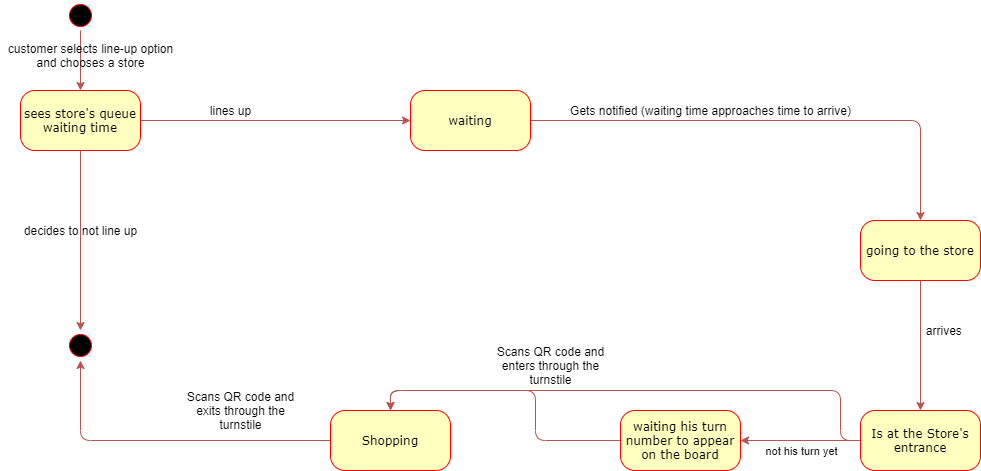
\includegraphics[width=\linewidth]{Customer_state.png}

\end{figure}

The first diagram shows the states relative to the \textbf{User} in the context of the line-up function.
\begin{figure}[H]



  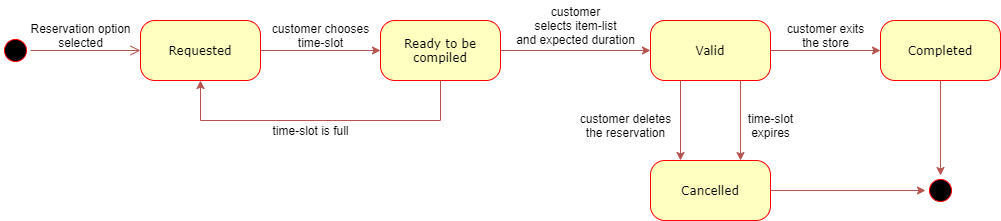
\includegraphics[width=\linewidth]{Reservation_state.png}


\end{figure}

The second diagram models the states in which a \textbf{Reservation} goes through in the context of the "booking a visit" function.\newline\newline\newline

\begin{figure}[H]

  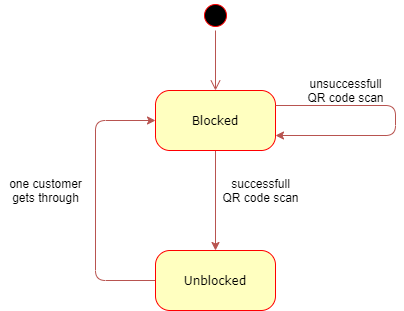
\includegraphics[width=6cm]{Turnstiles_state.png}


\end{figure}
The last one is a simple diagram, showing the functioning of the \textbf{Smart Turnstiles} positioned at the stores' entrances.

\subsection{Product Functions}
The main functions that the system will provide are listed in the following section. The identified high level requirements will be further broken down and detailed in section 3, with respect to the previously recognized goals of the system.
\subsubsection{Line up} 
As previously stated, the basic functionality allows users to virtually stand in line to enter the stores. Firstly, the user selects the store and chooses among the two available options: line up or book a visit. Whenever the choice is to line up, the system will show to the user the estimated waiting time to enter. At that point, if the user decides to actually get in the line, he/she will be asked to provide the expected duration of the visit and finally, he/she will receive the turn number and the QR code that has to be scanned when entering to the store. The user will be asked wether he/she will reach the store on foot or by car. While waiting, the user will be shown the passing of time, the calculated distance to the store and the estimated time he/she will need to get there (exploiting Google Maps API). The user will be notified by the system when the time he/she needs to get to the store equals the time left for the user to enter. Once arrived to the store, the user might need to wait few minutes until his/her number appears on the queue board. Finally, the smart turnstile will scan the QR code and unlock, letting the user enter the store and start shopping.
\subsubsection{Book a visit} 
As mentioned before, after choosing the store, the user also has the option to book a visit. He/she will select the preferred time slot and make a reservation whenever the slot is not already full. A QR code is generated and the user can access to the store at any moment of the time slot, as long as he/she exits before the end of it. When making the reservation, the user is asked to provide the expected duration of the visit and to select the categories of items that he/she intends to purchase. This last information is used by the system to understand which store’s department the customers are going to occupy in order to manage entrances in a finer way. In particular the system can either let more people in if the distribution is homogeneous inside the store or slow down the influx of people if customers are gathered in certain departments.
\subsubsection{Manage lines} 
The CLup system has to manage the lining up mechanism effectively. First of all, the waiting time assigned to customers that get in line, can change depending on several events. In particular, whenever a customer either gets out of the line or cancels a slot reservation, the system is able to decrease the waiting times of the users currently in line and optimize the influx of people. The waiting time can also decrease in the event that someone does not show up when his/her turn is arrived (there will be a fixed maximum delay tolerated by the system). Each user (for both the basic and advanced functionality) is asked to provide the expected amount of time they intend to spend inside the store, alternatively, users can choose to let the system infer that time (only if the system has enough data). Indeed, for each user, the system will collect and store informations about the duration of his/her visits and estimate an average. As a consequence, whenever a user’s visit lasts longer or less than the estimated time, the waiting time of the users in line can be optimized (increased or decreased). Ultimately, the system is also able to handle people who do not have access to the required technology. The store manager (or one of his employees) will print a number and a QR code for those who have to physically get in line and the system will take them into account when scheduling the next entrances (they will be assigned a fixed time of stay in the shop).
\subsubsection{Keep track of accesses} 
The CLup system is also meant to be used by store managers to keep track of entrances in their buildings. This is possible thanks to the smart turnstiles that scan the QR codes and let people in or out (only if the QR code is not expired or false). Consequentially, a customer counter is updated  so that stores managers can check whether their store’s capacity is respected.
\subsection{User Characteristics}
The application is supposed to be used by the following actors:
\begin{enumerate}
\item\textbf{Registered user}: someone who downloaded the application on his/her device, registers to CLup and uses its services.\medskip\\
Depending on the service used, the following distinction can be done: 
\begin{itemize}
\item Line up: the user is someone that wants to enter the store as soon as possible and might not live too far from it. Indeed, he/she prefers to line up and is ready to move even if the waiting time is shortened.
\item Book a visit: the user is someone who plans on visiting the store in advance and at a fixed time.
\end{itemize}
\item\textbf{Unregistered user}: someone who do not have access to the required technology and therefore is not registered to CLup services. The only way in which he/she interacts with the system is by physically retrieving a turn number and a QR code from the ticket dispenser located at the store. The system will take into account this actor when scheduling the next entrances
\item\textbf{Store manager}: someone who is responsible for managing a store and registers to CLup to monitor the influx of people in his/her building.
\end{enumerate}
\subsection{Constraints}
The system will have to ask users' permission to retrieve and use their positions without storing them. Moreover, the collection and treatment of personal data must comply with the principles and rules of the General Data Protection Regulation.
\subsection{Assumptions and Dependancies}
\subsubsection{Domain assumptions}
\noindent\medskip
[D1] - GPS provides the exact location with an error of 5 meters at most.\\
\noindent\medskip
[D2] - The time calculated from Google Maps to reach the store is correct.\\
\noindent\medskip
[D3] - The user does not to arrive earlier than the indicated time.\\
\noindent\medskip
[D4] - The user follows the shortest path to the store, without making deviations and stops.\\
\noindent\medskip
[D5] - Each reservation is meant to be for one and only one person.\\
\noindent\medskip
[D6] - The turnstiles let you in or out only if the scanned QR code is valid.\\
\noindent\medskip
[D7] - The user does not change location while is waiting for his/her turn.\\
\noindent\medskip
[D8] - The user does not change the indicated means of transport.\\
\noindent\medskip
[D9] - The user respects slots' time boundaries.\\
\noindent\medskip
[D10] - The user respects social distancing inside the store.\\

\section{Specific Requirements}
\subsection{External Interface Requirements}
\subsubsection{User Interfaces}
\subsubsection{Hardware Interfaces}
\subsubsection{Software Interfaces}


\subsection{Functional Requirements}
\subsubsection{List of Requirements}
\subsubsection{Mapping}
\subsubsection{Scenarios}
\medskip
\textbf{Scenario 1: Line up}\medskip\\
Mario is a 40 years old teacher living in Pisa. During the weekend, he wants to take advantage of some free time to go grocery shopping for the coming week. Since the covid-19 pandemic is getting worse, he does not want to risk ending up in crowded lines or stores. Therefore, he decides to exploit the virtual lining service, offered by CLup application on his smartphone. He chooses the nearest Eurospin on the app and finds out that the waiting time is 40m 32s. He decides to get in line and selects “on foot” as means of transport, to get some fresh air. He wants to do a lot of shopping, so he indicates an hour as estimated time to spend inside the store. After approximately 15 min, Mario receives a notification from CLup saying that it’s time to leave and therefore, he prepares for his 20 min walk to reach the store. Once arrived, he sees his number on the board, he selects the QR code on his smartphone to have it scanned by the turnstile at the entrance and, finally, he starts shopping.\medskip\\
\medskip
\textbf{Scenario 2: Get out of line}\medskip\\
Elisa is a young mum of two kids who decides to go shopping for Christmas’ presents on a Wednesday morning, while her children are at school. Considering that Christmas is coming, she expects to find many people shopping and so she decides to use the CLup application to get in the line of her favorite gift shop. The current waiting time is such that she will be perfectly in time to pick her kids up from school. Unfortunately, it seems like some store’s departments are particularly crowded, or maybe some customers are staying inside more than they should. As a result, Elisa’s waiting time has increased a little and she realizes she would be late for the end of school. In the end, she gets out of the line and decides to try again the following day. \medskip\\
\medskip
\textbf{Scenario 3: Book a visit}\medskip\\
Anna is a single 36 years old business woman currently living in Milan. She has a very busy schedule and therefore she cannot risk wasting too much time buying groceries. For this reason, she often uses CLup application on her smartphone to book visits to her usual supermarket. On Tuesday, she will be getting off work at 4 pm and she has exactly two hours, before a late afternoon video call. Among the available time slots, she chooses the one from 5:30 pm till 6:30 pm, as she is sure she will not need to stay inside for more than half an hour. Last time she went to the supermarket, it took her 20 min to do the shopping, so she selects that same duration, shown by the system, for her Tuesday’s visit as well. Lastly, she select the categories of products that she intends to purchase and confirms the whole reservation.\medskip\\
\medskip
\textbf{Scenario 4: Cancel a reservation}\medskip\\
Giorgio is a young man working as a consultant in Turin. While he’s in the office, he decides to make a reservation to go to the supermarket later in the afternoon, because he wants to surprise his wife with the grocery. He uses CLup application to book the visit for the preferred time slot. At lunch time, Giorgio’s wife, who does not trust her husband’s sense of initiative, calls Giorgio to inform him that she is going grocery shopping. At this point, the poor Giorgio is forced to cancel his booked visit. He opens CLup app, goes in the “My Reservations” section and cancels his last reservation.\medskip\\
\medskip
\textbf{Scenario 5: Customer without a smartphone gets a ticket}\medskip\\
Antonio is a 71 years old retired man who lives in Monza during the period of lockdown, due to the COVID-19 pandemic. Antonio is reluctant to technology and in fact, the cellphone he owns is suitable only for basic functionalities. For this reason, he is not able to download CLup’s application and use its services. He needs to go grocery shopping, so he walks up to the nearest supermarket. He reaches the info desk and finds out that there is a virtual lining mechanism going on and that he will have to wait for his turn at the entrance. Angela, a store’s employee who is responsible for taking care of customers who do not have access to the required technology, accesses to CLup’s WebApp from her computer and prints for Antonio a ticket, with a turn number and a QR code. She explains to him how and where to scan the QR code as soon as his turn number appears on the led board at the entrance.\medskip\\
\medskip
\textbf{Scenario 6: Check customer counter}\medskip\\
Paola is the manager of a big Esselunga store in Milan. During the day, she periodically checks that everything is proceeding as planned. In particular, she takes a look at each store department to make sure that there are no crowds and she also checks the number of people currently in the store. To do so, she accesses CLup’s WebApp from her office’s computer and clicks on “Check customer counter” button. In this way, she is always able to verify whether the CLup system is efficiently working, without violating the maximum capability of her store.\medskip\\
\subsubsection{Use cases}
\subsubsection{Use cases Diagrams}
\subsubsection{Sequence Diagrams}

\begin{figure}[H]
  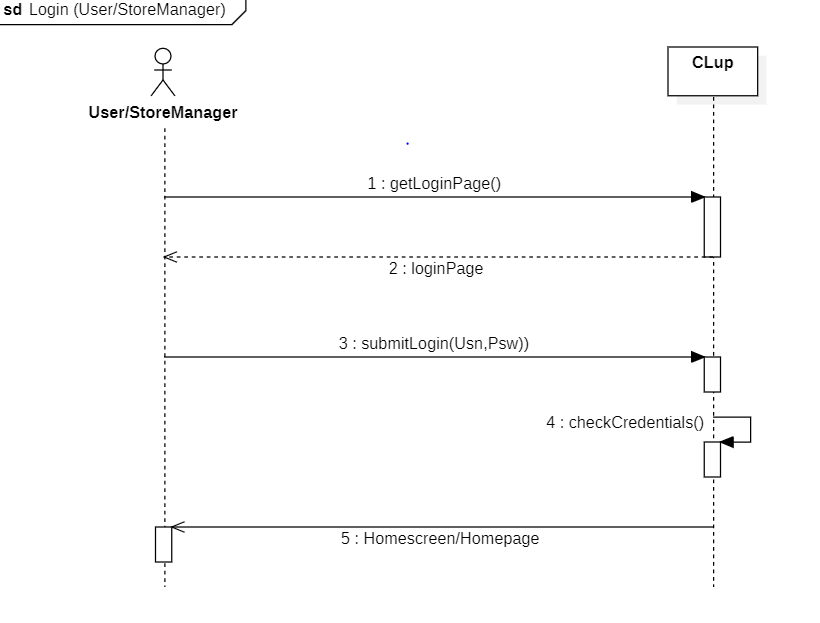
\includegraphics[width=\linewidth]{LoginSequence.png}
  
\end{figure}

\begin{figure}[H]
  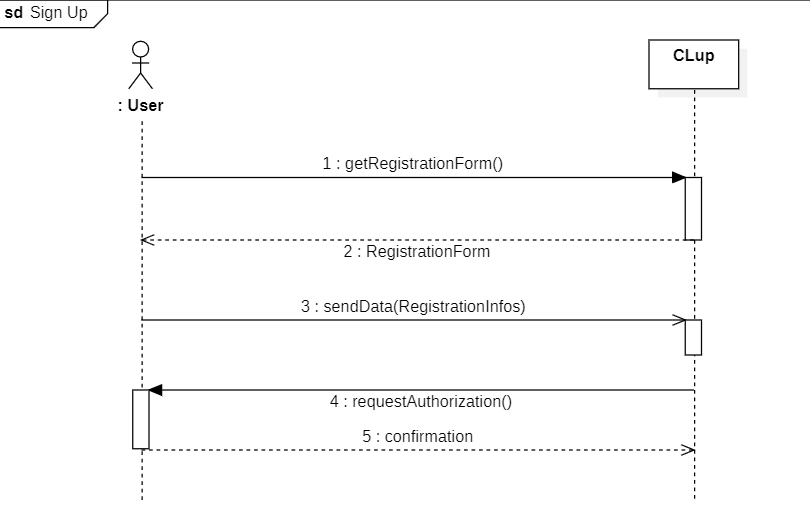
\includegraphics[width=\linewidth]{SignUpSequence.png}
  
\end{figure}

\begin{figure}[H]
  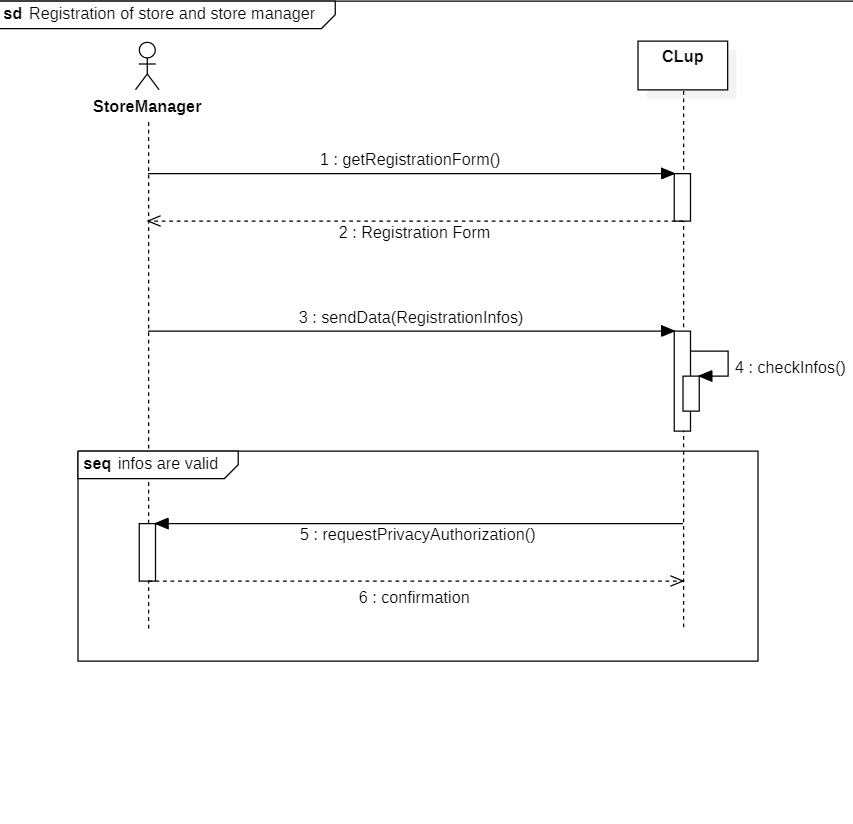
\includegraphics[width=\linewidth]{RegistrationSequence.png}
  
\end{figure}

\begin{figure}[H]
  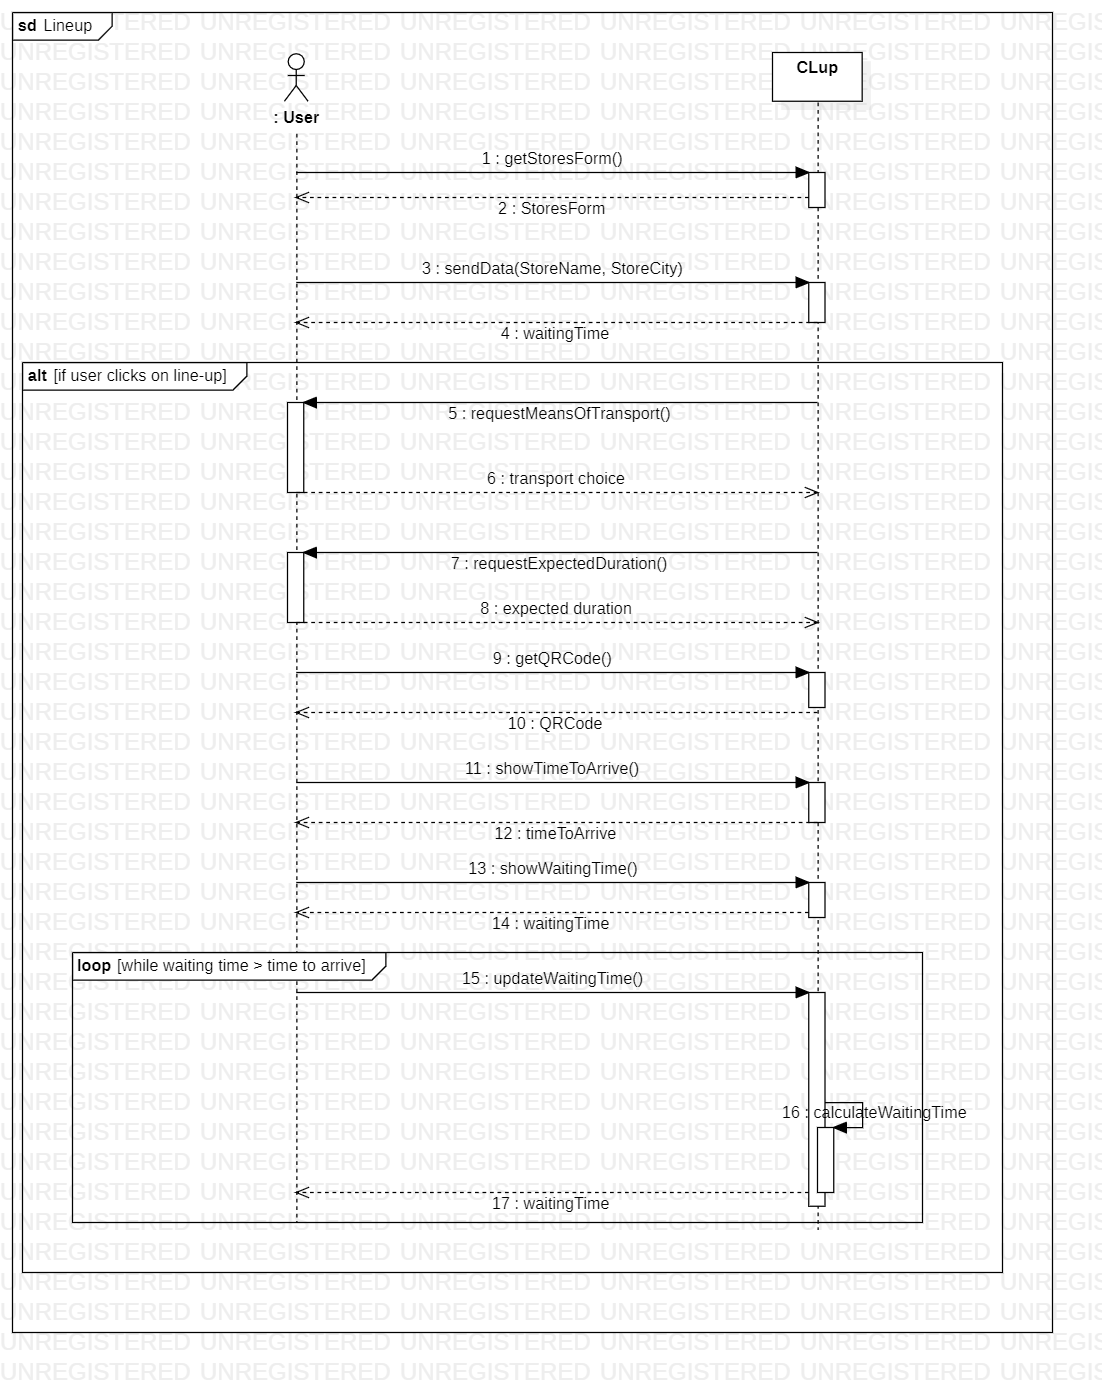
\includegraphics[width=\linewidth]{LineUpSequence.png}
  
\end{figure}

\begin{figure}[H]
  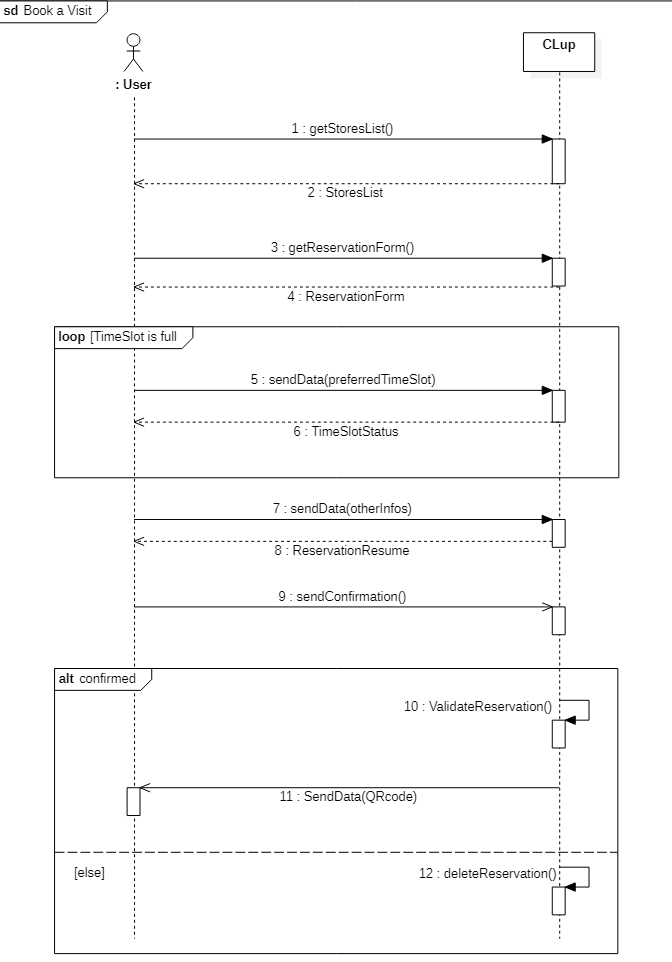
\includegraphics[width=\linewidth]{BookSequence.png}
  
\end{figure}

\begin{figure}[H]
  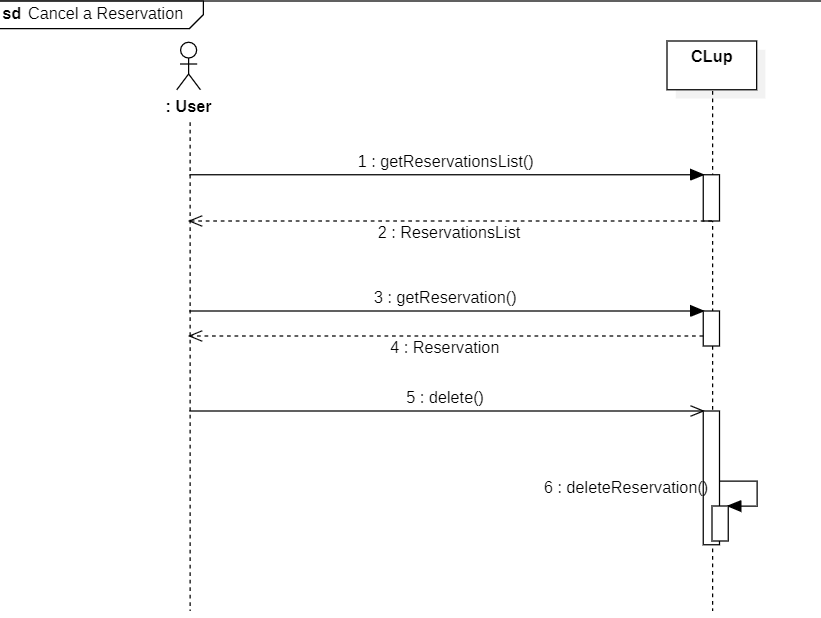
\includegraphics[width=\linewidth]{CancelReservationSequence.png}
  
\end{figure}

\begin{figure}[H]
  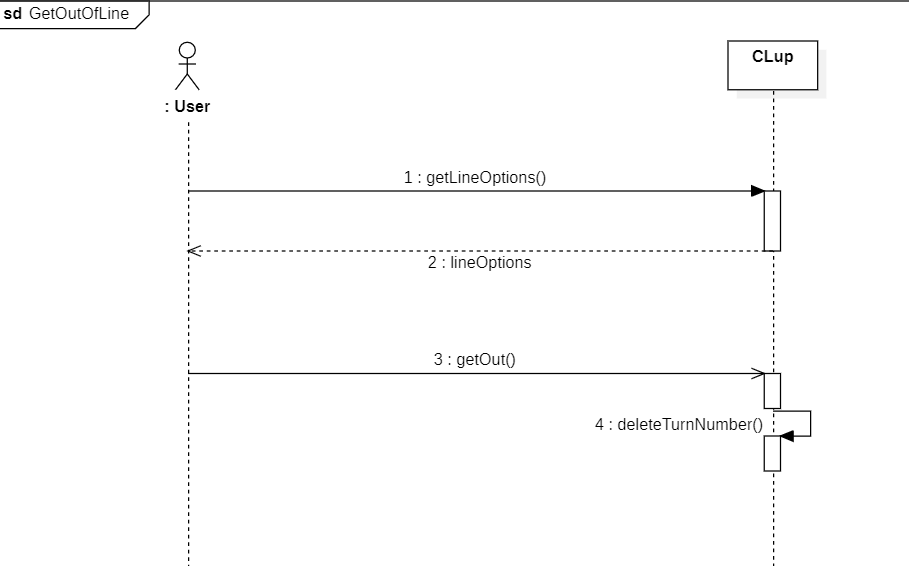
\includegraphics[width=\linewidth]{OutOfLineSequence.png}
  
\end{figure}

\begin{figure}[H]
  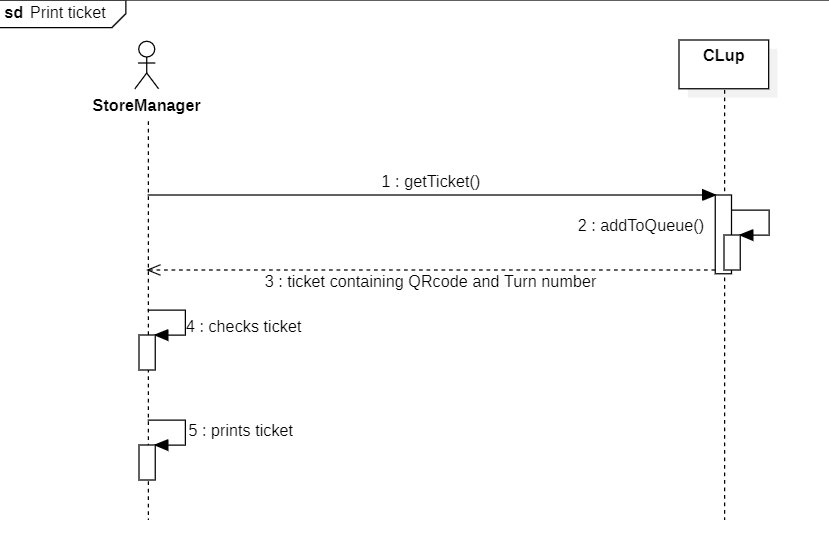
\includegraphics[width=\linewidth]{PrintTicketSequence.png}
  
\end{figure}

\begin{figure}[H]
  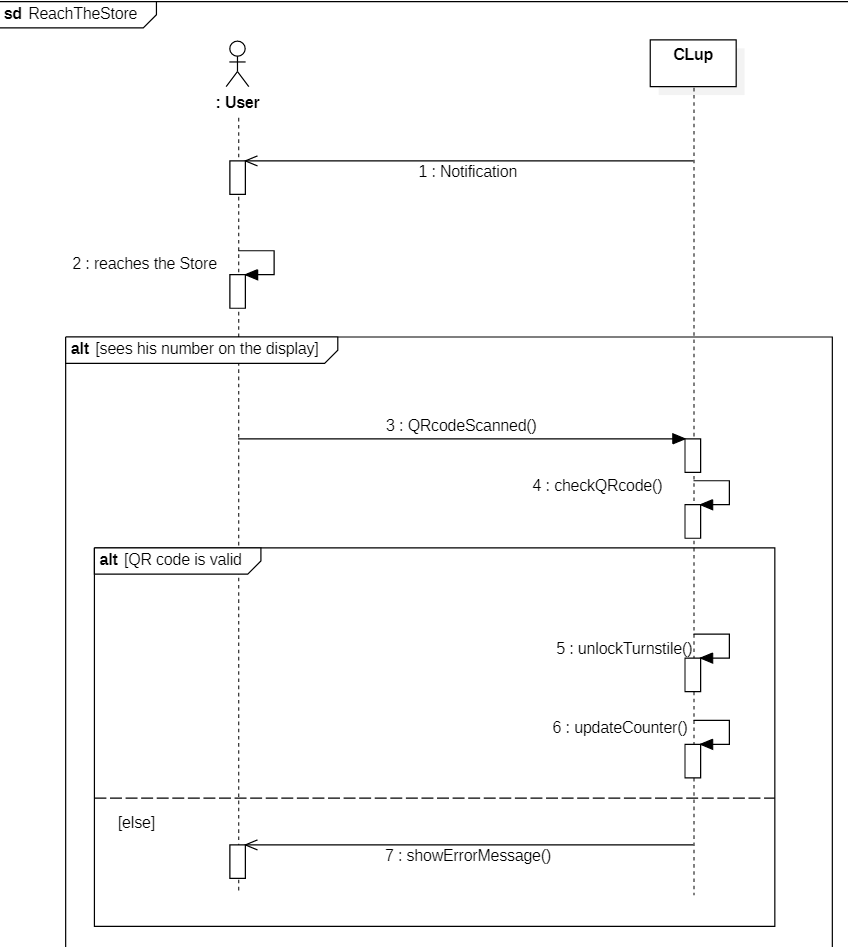
\includegraphics[width=\linewidth]{ReachStoreSequence.png}
  
\end{figure}




\subsection{Performance Requirements}

\subsection{Design Constraints}
\subsubsection{Standards compliance}
\subsubsection{Hardware limitations}
\subsubsection{Any other constraints}

\subsection{Software System Attributes}
\subsubsection{Reliability}
\subsubsection{Availability}
\subsubsection{Security}
\subsubsection{Maintainability}
\subsubsection{Portability}
\subsubsection{Scalability}
\subsubsection{Compatibility}

\subsection{Additional Specifications}



\end{document}